\section{Process mining}
\label{sec:process_mining}

We mined the logs generated by the simulation of the collapsed workflow.

We modified the simulation configuration 

\begin{figure}[H]
\centering
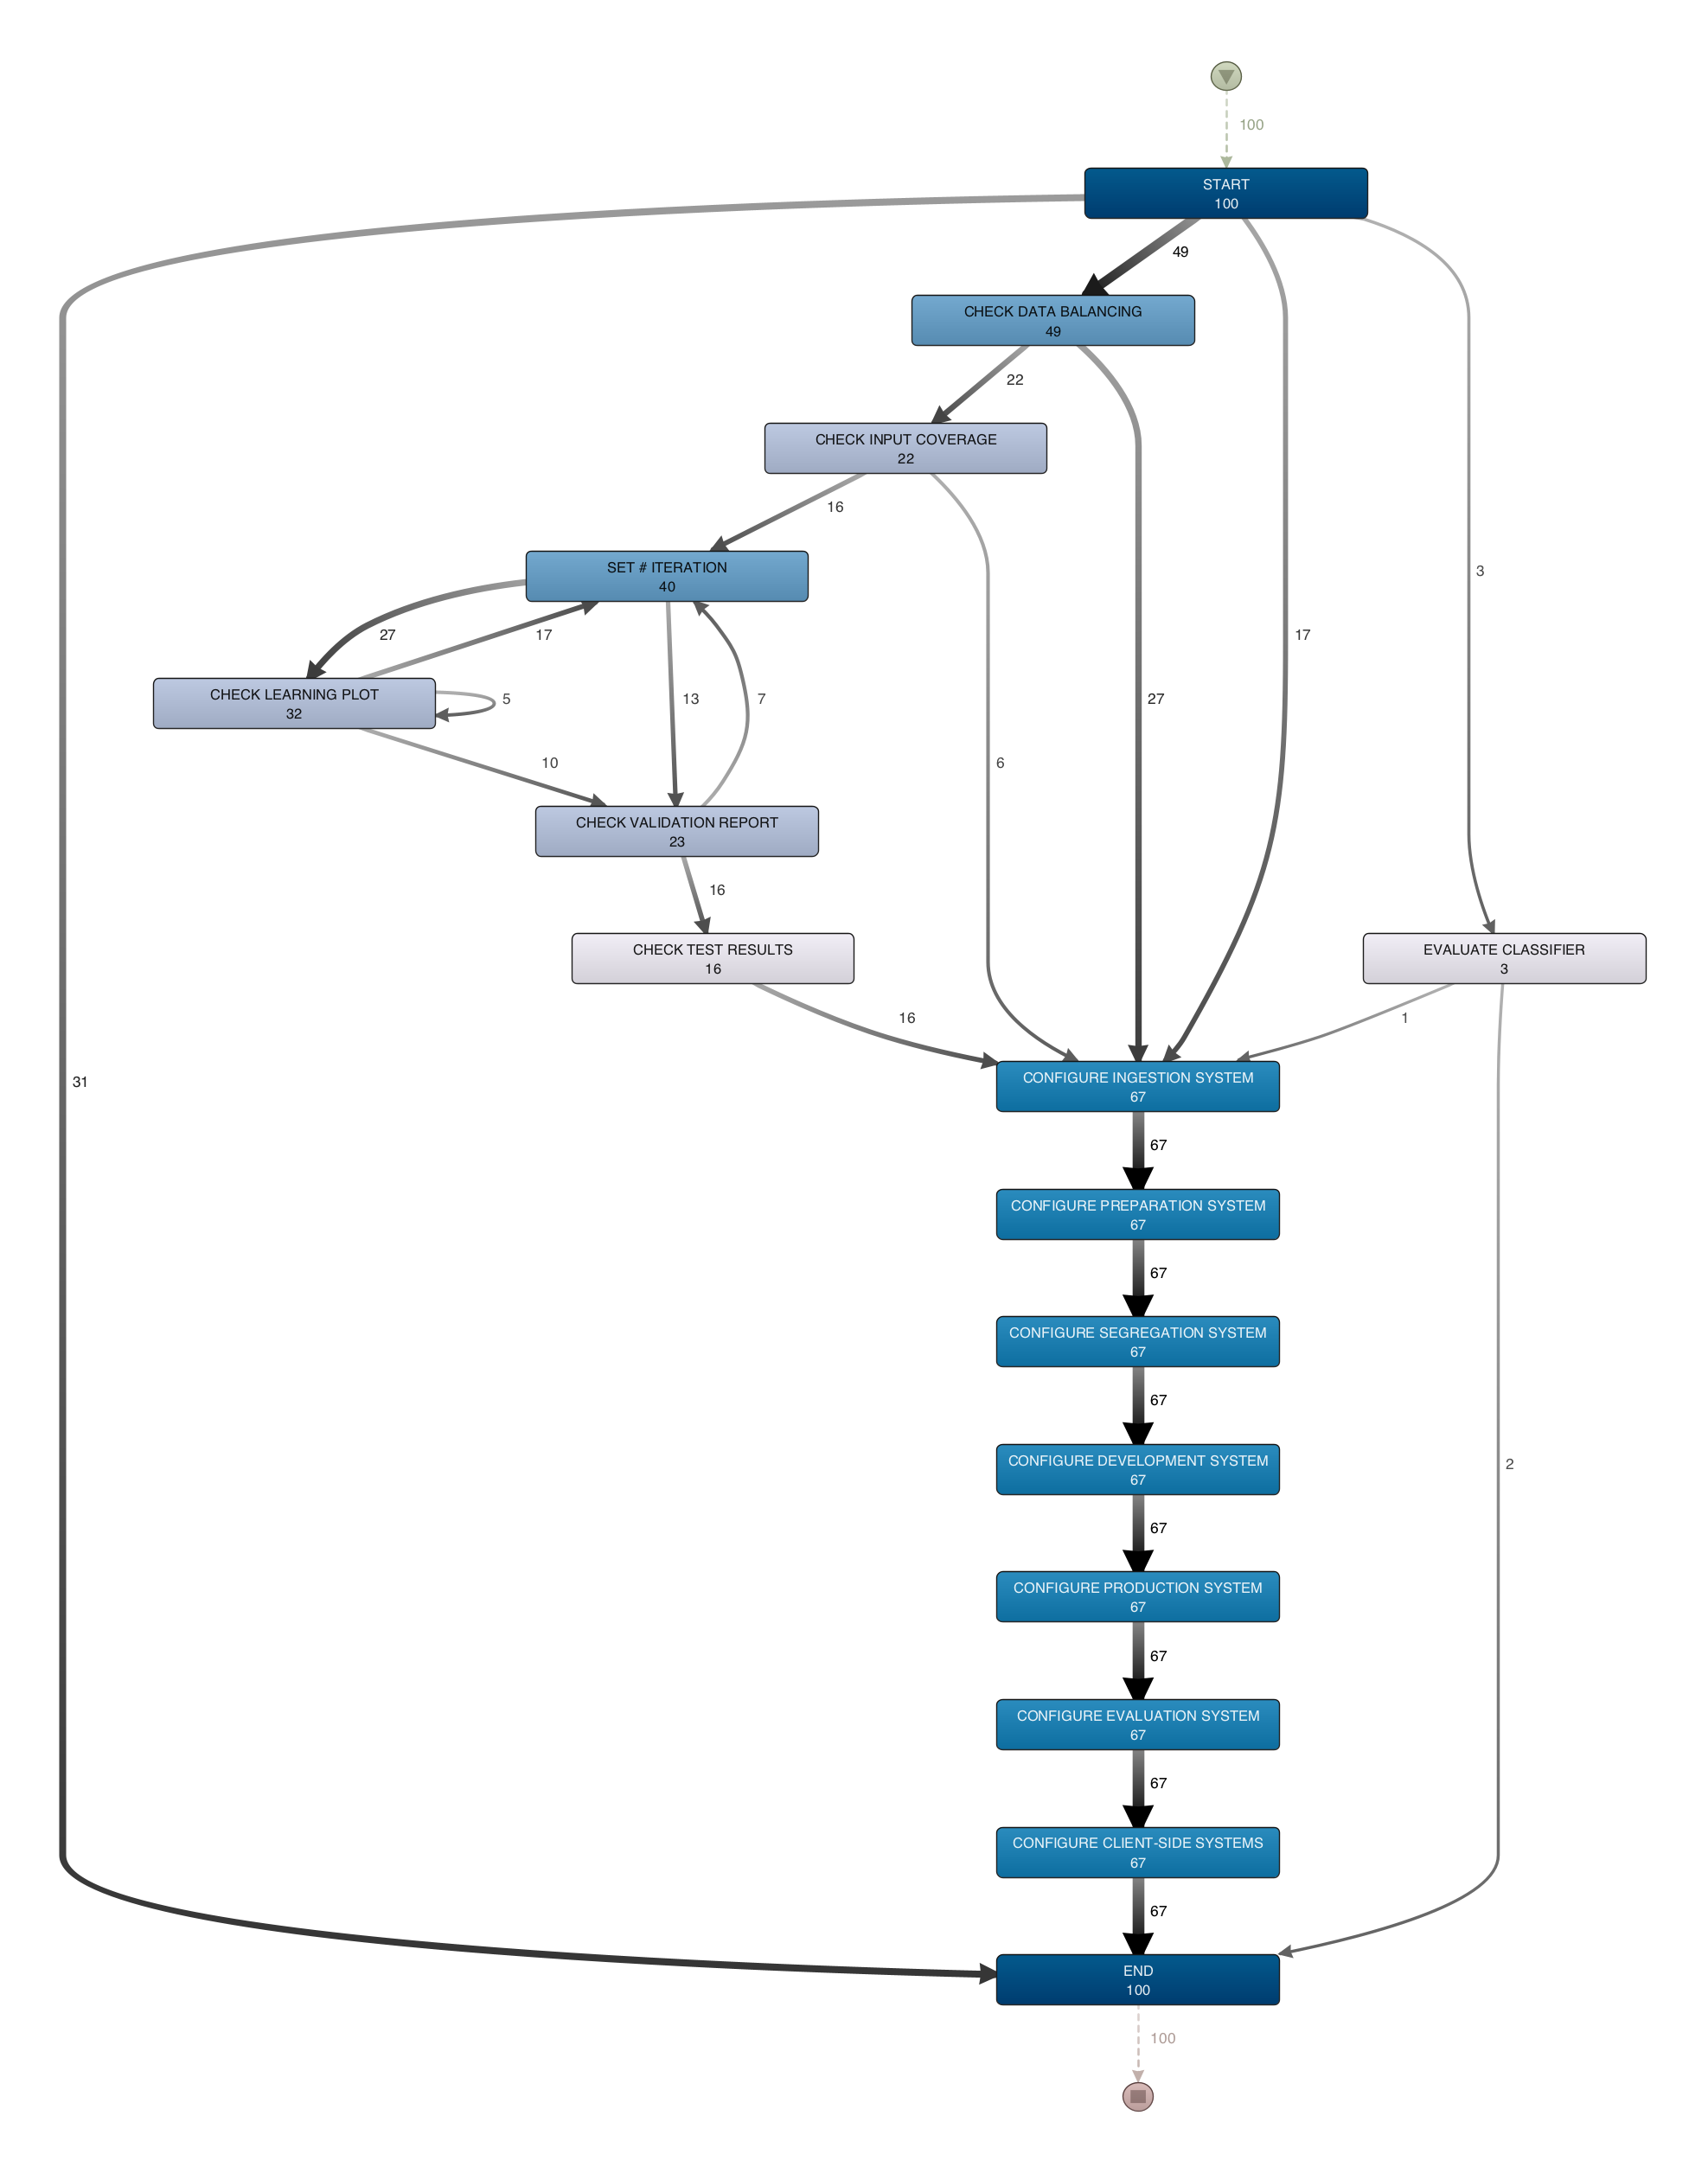
\includegraphics[width=0.8\textwidth]{figures/disco_map.png}
\caption{Disco analysis}
\label{fig:disco_analysis}
\end{figure}

\begin{figure}[H]
\centering
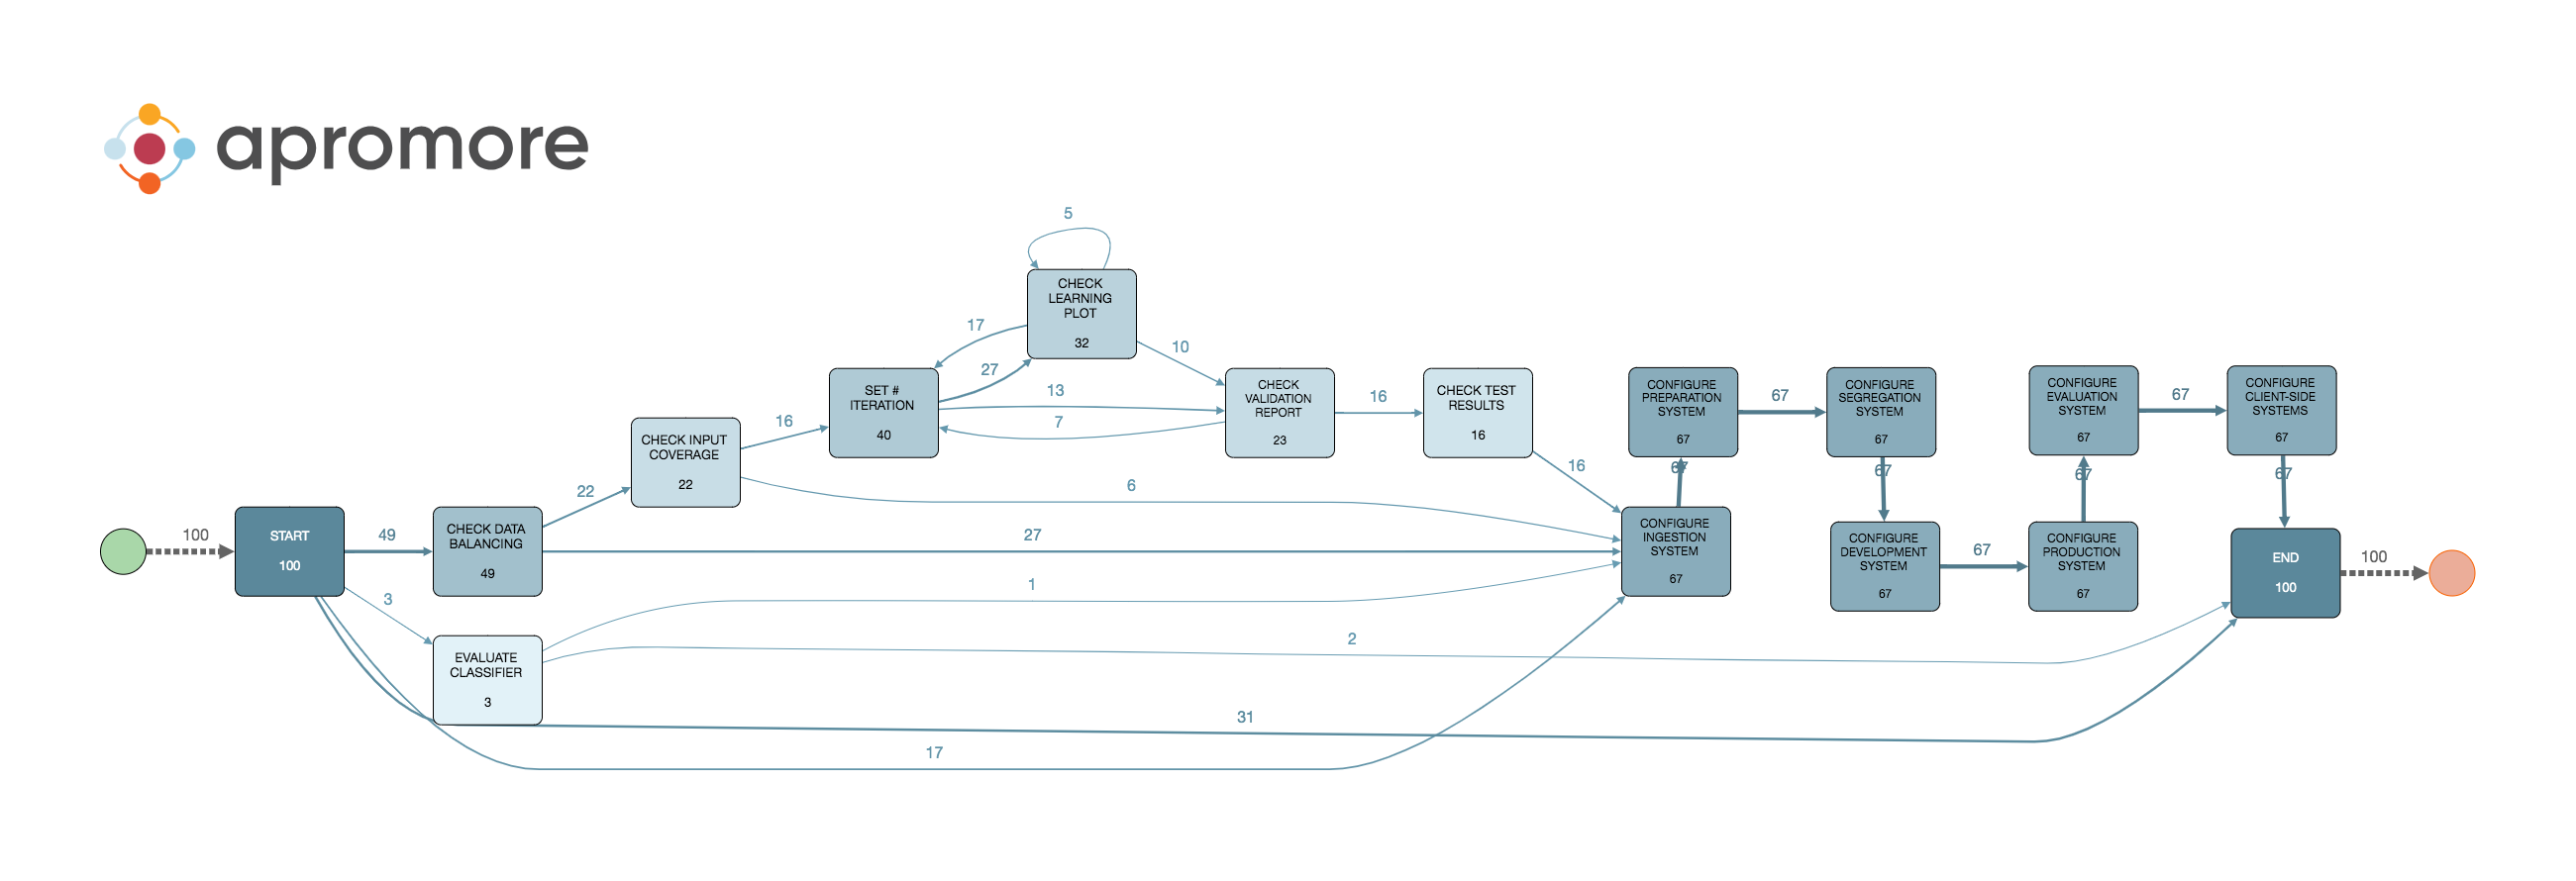
\includegraphics[width=\textwidth]{figures/apromore_map.png}
\caption{Apromore analysis}
\label{fig:apromore_analysis}
\end{figure}

As we can see, the two transition maps mined from Disco and from 
Apromore are identical.

\begin{figure}[H]
\centering
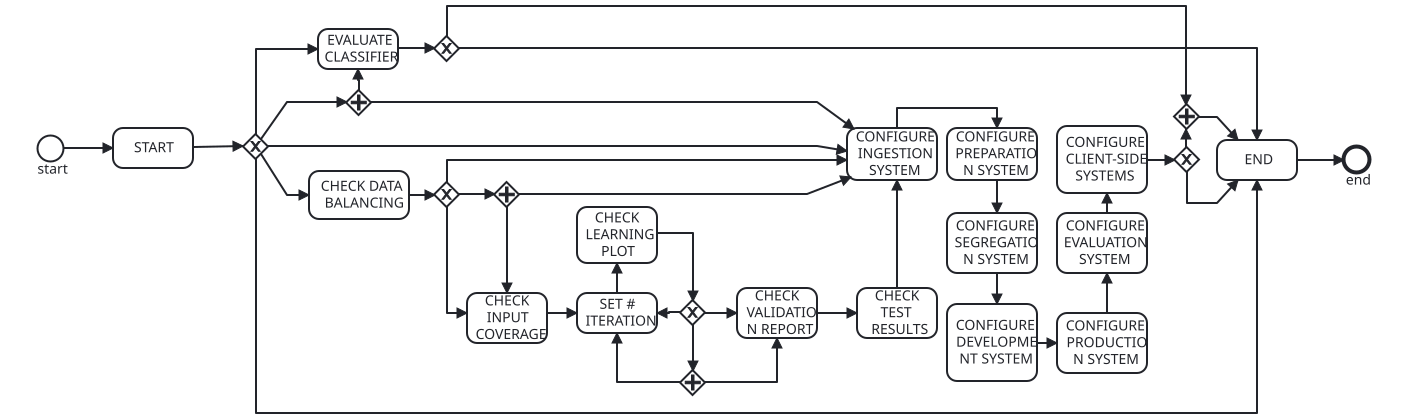
\includegraphics[width=\textwidth]{figures/prom_mined.png}
\caption{ProM mined BPMN model}
\label{fig:prom_mined}
\end{figure}

The BPMN model mined from ProM is not compliant with the BPMN 2.0 specification
(section 10.5). Furthermore, the model contains parallel gateways that are never present
in the collapsed model.

\begin{figure}[H]
\centering
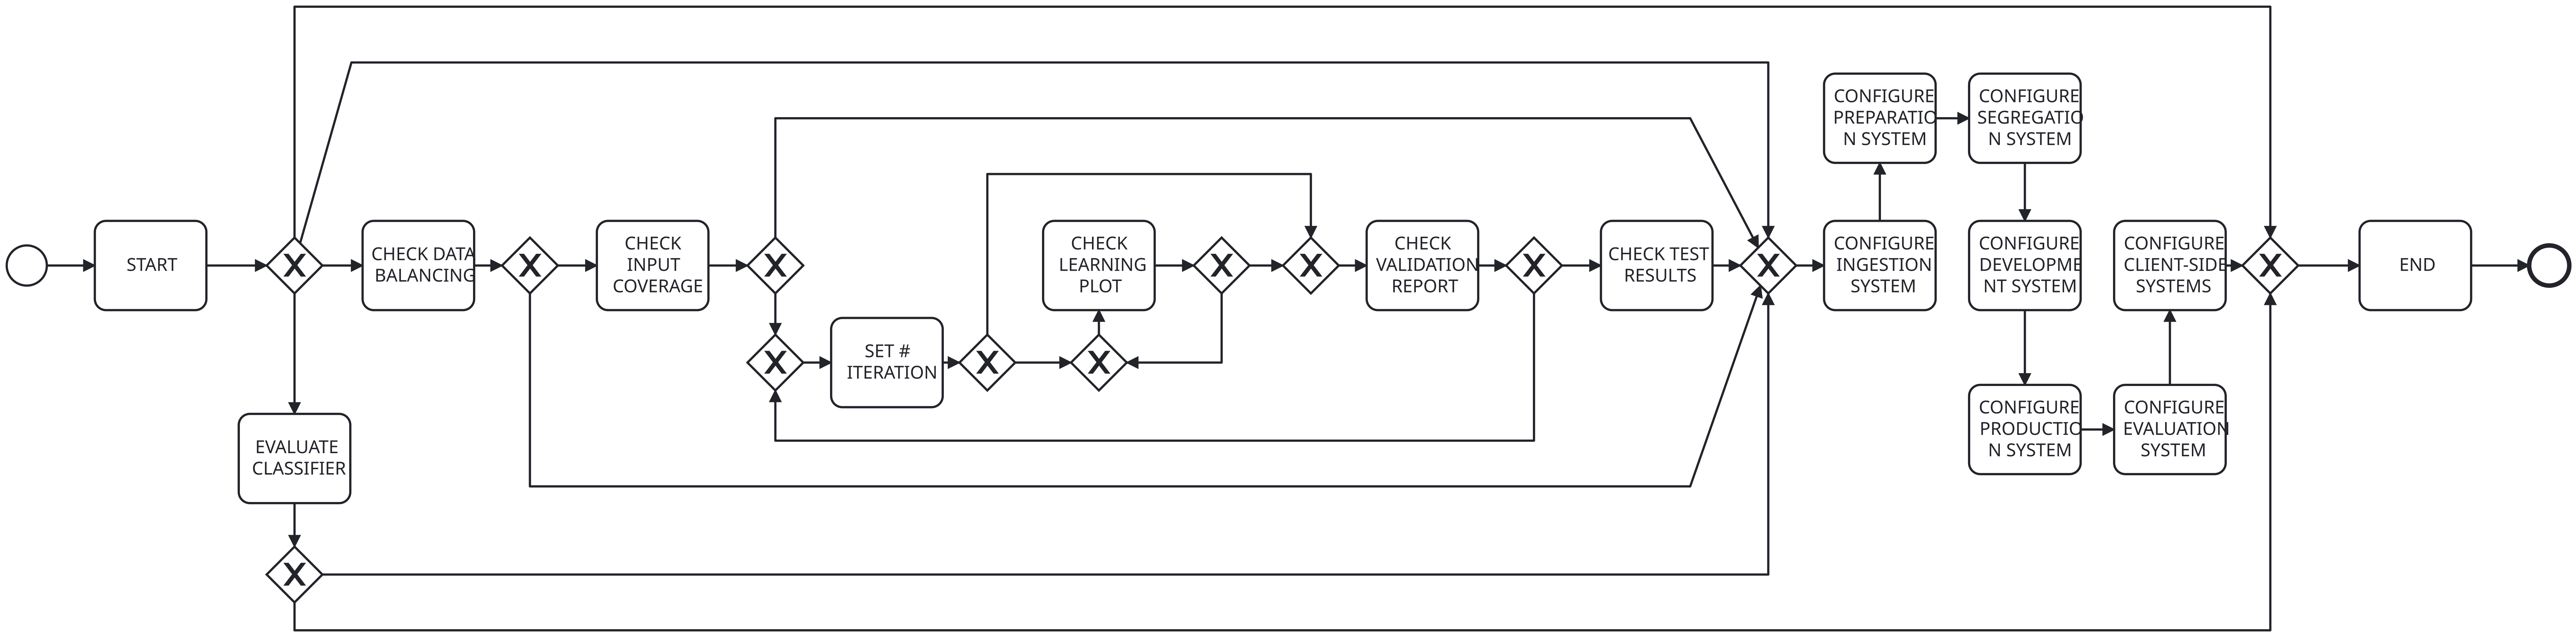
\includegraphics[width=\textwidth]{figures/apromore_mined.png}
\caption{Apromore mined BPMN model}
\label{fig:apromore_mined}
\end{figure}

The BPMN model mined from Apromore is much more sensible compared to the one from ProM, also
it is compliant with the BPMN 2.0 specification.

\begin{table}[H]
\centering
\begin{tabular}{|r|l|l|l|l|}
\hline
\textbf{Tool} & \textbf{Trace} & \textbf{Generalization} & \textbf{Precision} & \textbf{Simplicity} \\
\hline
Apromore & 0.4203 & 0.9872 & 0.7566 & \\
\hline
ProM & 0.6666 & 0 & 0 & \\
\hline
\end{tabular}
\caption{Comparison of the process mining tools}
\label{tab:process_mining_comparison}
\end{table}